%%%%%%%%%%%%%%%%%%%%%%%%%%%%%%%% 
\section{The Slow-Control System} 
\label{sec:detectors-fd-alt-dcs}

\fixme{A sentence about what it is and what it controls would be nice. Can we say ``the slow-control monitoring system''?}
The slow-control system for the far detector is part of a continued,
progressive prototyping effort aimed at developing a control system
dedicated to multi-kiloton LAr dual-phase detectors. It has
been designed in the framework of the LAGUNA-LBNO design study and 
the WA105 experiment, following the successful example and the
expertise developed in the context of the ArDM
experiment~\cite{Badertscher:2013ygt}. ArDM is currently operating one
ton of LAr \fixme{a one-ton LArTPC?} in an underground laboratory (LSC, Spain). This \fixme{the ArDM or the LBNO design that WA105 will test?}
slow control system introduces %for the first time 
the use of
National Instruments Compact RIO (Reconfigurable Input Output) modules
for acquisition of all the physical quantities of interest. 
Figure~\ref{fig:NI_proto} shows a rack prepared for the WA105
3$\times$1$\times$1~m$^3$ prototype that is ready to be tested at CERN.

\begin{cdrfigure}[Slow Control prototype rack]{NI_proto}{The rack is a 
prototype of the entire Control System; it  embeds modules for resistive 
temperature sensors, pressure  sensors, strain gauges, liquid argon level 
meters, control for  heaters. On the upper part a redundant 24 V power supply 
provides fault tolerant power to the National Instrument controller and modules. 
Calibration of modules and sensors is ongoing.}
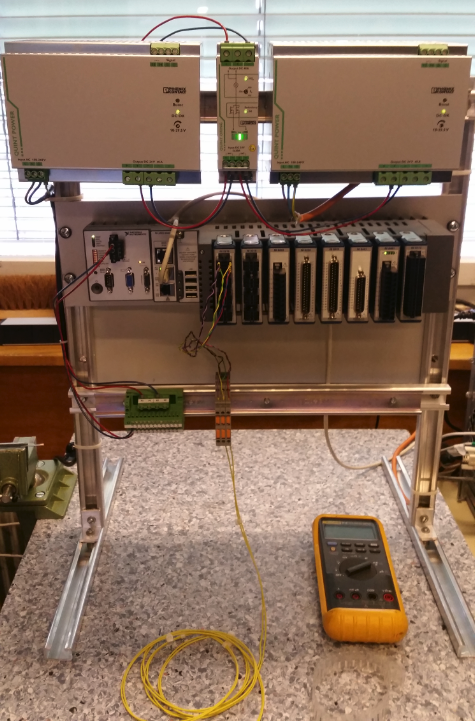
\includegraphics[scale=0.4, angle=0]{rack_2.jpg}
\end{cdrfigure}

The slow-control system %of the far detector and 3$\times$1$\times$1~m$^3$ prototype detectors 
is designed to monitor
the following physical quantities inside the tank:
\begin{itemize}
 \item temperatures (with platinum resistors)
 \item pressures (with commercial piezoelectric sensors)
 \item LAr levels (with custom-made capacitive sensors and electronics)
 \item deformations of materials (with resistive strain gauges)
\end{itemize} 

%Moreover, 
In addition, the slow control system provides the hardware infrastructure
needed to monitor traces of O$_2$, N$_2$ and H$_2$O impurities in the tank, to
monitor and control the high- and low-voltage power supplies, heaters,
lighting system and cryogenic cameras video system.\fixme{can we just say ``cryogenic video system''?} It will also
interface to the cryogenic system and to the motorized system that
adjusts the position of each Charge Readout Plane (CRP).

The entire slow-control system of the WA105 demonstrator will be
managed through a single LabView interface \fixme{citation?} which will provide access
to all the sensors, control the actuators and provide the platform for
the video %-cameras 
monitoring system both inside and outside the tank. 
%overlying supervisory
Higher-level software will be implemented in the CERN UNICOS
(UNified Industrial Control System) framework~\cite{unicos} to
provide the operator interface for the monitoring of all the
physical quantities and the handling of alarms. %, as is commonly done in CERN experiments.

As discussed in Section~\ref{sec:detectors-fd-ref-ov}, the
charge-readout system %of the far detector 
is implemented via CRP
modules of 3$\times$3~m$^2$. Each %3$\times$3~m$^2$ 
CRP is an
independent detector, hence its instrumentation can also be treated as
independent. A complete list of the sensors planned %which are been foreseen 
for use in both the %3$\times$3 m$^2$
DUNE far detector and the
3$\times$1$\times$1~m$^3$ WA105 prototype is provided in
Table~\ref{fig:sc_sensors}. 
\begin{cdrfigure}[Dual-phase slow control sensors.]{sc_sensors}
{List of the slow control sensors for the 3$\times$1$\times$1~m$^3$ WA105 prototype and far detectors CRP}
 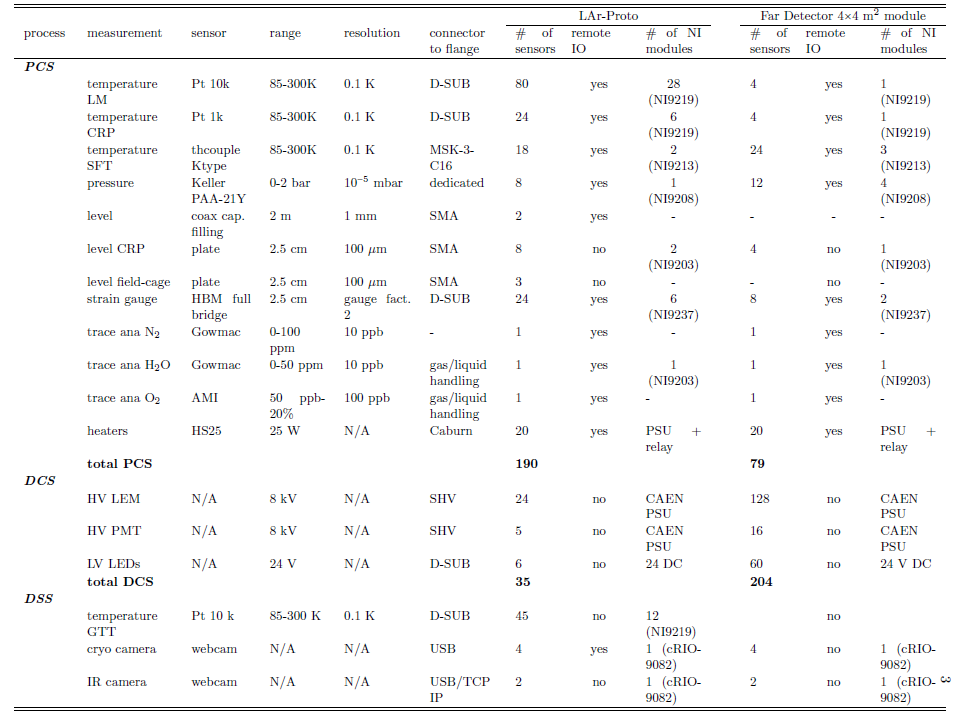
\includegraphics[scale=0.6, angle=0]{sc_table.png} %[scale=0.52, angle=0]{sc_table.png}
 \end{cdrfigure}
The number of sensors for the
far detector CRP is extrapolated from the number for % of the sensors foreseen
the %3$\times$1$\times$1~m$^3$ 
prototype and is not yet final.
The sensor instrumentation of the %$3$\times$1$\times$1~m$^3$ 
WA105
prototype has also led to the design of a custom Slow-Control
Feedthrough (SCFT), based on the use of weldable connectors for high
vacuum (see Figure~\ref{fig:SC_flange}). A specific SCFT for the DUNE 
3$\times$3~m$^2$ CRP would be based on this design.
\begin{cdrfigure}[Slow control feedthroughs]{SC_flange}{The 3 SCFTs providing 
weldable connectors for all the instrumentation inside the 3$\times$1$\times$1~m$^3$  WA105 tank. 
The number of sensors per module in the DUNE far detector will be drastically 
reduced with respect to this WA105 prototype.}
  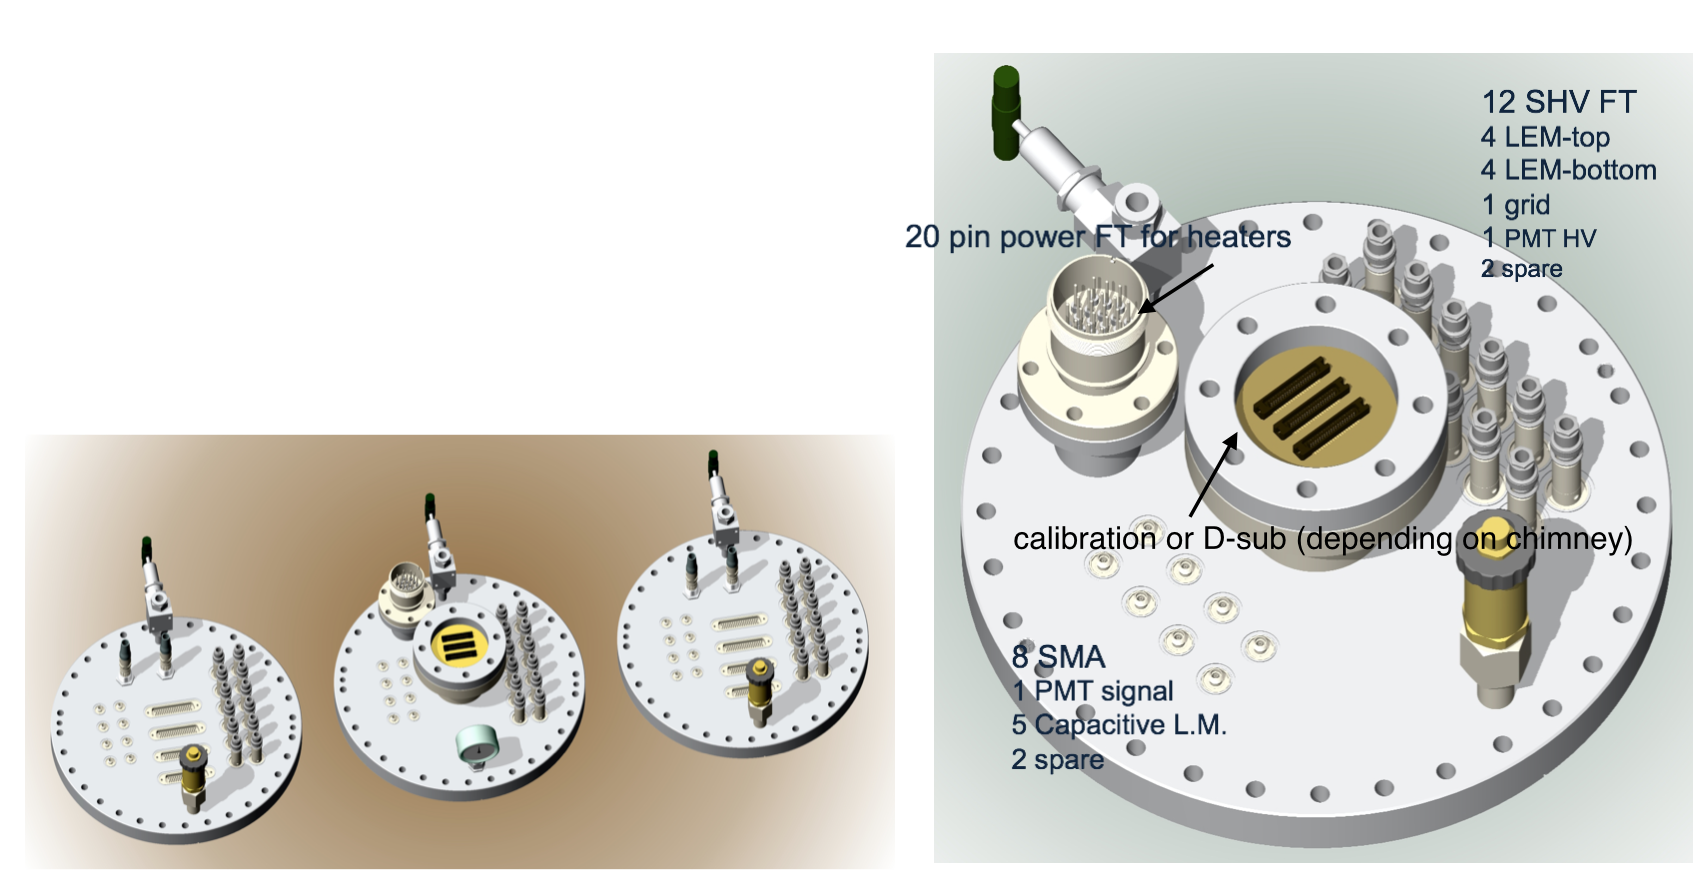
\includegraphics[scale=0.52, angle=0]{SC_flange.png}
 \end{cdrfigure}
